% !TEX root = ./main.tex

% ---------------- Macros ----------------
% Colors
\definecolor{OutdoorDark}{rgb}{0,.5,0}
\definecolor{IndoorDark}{rgb}{0,0.3,0.8}
\definecolor{SubTDark}{rgb}{0.5,.27,0.11}
\definecolor{AerialDark}{rgb}{.5,.0,.5}
\definecolor{UnderWaterDark}{rgb}{0.16, 0.46, 0.81}
\colorlet{Outdoor}{OutdoorDark!20!white}
\colorlet{Indoor}{IndoorDark!20!white}
\colorlet{SubT}{SubTDark!20!white}
\colorlet{Aerial}{AerialDark!20!white}
\colorlet{UnderWater}{UnderWaterDark!20!white}
\colorlet{OutdoorLight}{OutdoorDark!70!white}
\colorlet{IndoorLight}{IndoorDark!70!white}
\colorlet{SubTLight}{SubTDark!70!white}
\colorlet{AerialLight}{AerialDark!70!white}
\colorlet{UnderWaterLight}{UnderWaterDark!70!white}
% Symbols
\newcommand{\symbolHt}{1.2em}
\newcommand{\oppsymbolHt}{1em}
\newcommand{\outdoorChar}{%
    \begingroup\normalfont
    
\includegraphics[height=\symbolHt]{symbols/outdoor.png}%
    \endgroup
}
\newcommand{\indoorChar}{%
    \begingroup\normalfont
    
\includegraphics[height=\symbolHt]{symbols/indoor.png}%
    \endgroup
}
\newcommand{\subtChar}{%
    \begingroup\normalfont
    
\includegraphics[height=\symbolHt]{symbols/cave.png}%
    \endgroup
}
\newcommand{\hawkinsChar}{%
    \begingroup\normalfont
    
\includegraphics[height=\symbolHt]{symbols/degraded.png}%
    \endgroup
}
\newcommand{\aerialChar}{%
    \begingroup\normalfont
    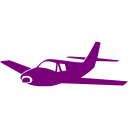
\includegraphics[height=\symbolHt]{symbols/aerial.png}%
    \endgroup
}
\newcommand{\underwaterChar}{%
    \begingroup\normalfont
    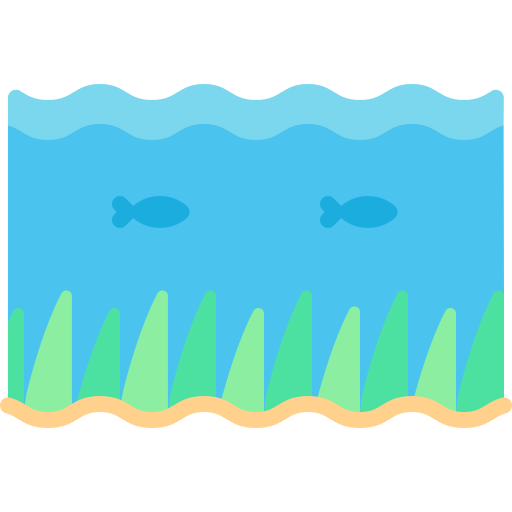
\includegraphics[height=\symbolHt]{symbols/underwater.png}%
    \endgroup
}
\newcommand{\viewpointChar}{%
    \begingroup\normalfont
    
\includegraphics[height=\symbolHt]{symbols/viewpoint.png}%
    \endgroup
}
\newcommand{\lightingChar}{%
    \begingroup\normalfont
    
\includegraphics[height=\symbolHt]{symbols/day_night.png}%
    \endgroup
}
\newcommand{\oppositeChar}{%
    \begingroup\normalfont
    
\includegraphics[height=\oppsymbolHt]{symbols/opp_viewpoint.png}%
    \endgroup
}
% ----------------------------------------


Prior Visual Place Recognition (VPR) methods have shown great
performance when tackling task-specific challenges in isolation. A
generic out-of-the-box model will need to perform adequately well
under a large set of challenges, including cases where there isn't
enough data for training or when training on different domains is
complex. This chapter introduces AnyLoc \cite{Keetha2023AnyLocTU}
which is the first step towards a universal VPR system.

VPR task is defined in \cref{subsec:intro-vpr}. AnyLoc aims to solve
image retrieval over a wide range of dataset settings using an
off-the-shelf foundation model without any VPR-specific fine-tuning.

\section{Prior Knowledge}

\subsection{VPR Baselines}

Global image descriptors are already described in
\cref{subsec:intro-vpr}. We choose to compare with the following
prominent baselines that are widely used in the VPR community.

\paragraph{NetVLAD \cite{Arandjelovi2015NetVLADCA}} is a smooth
(differentiable) version of VLAD (Vector of Locally Aggregated
Descriptor). It is a weakly supervised contrastive learning method
where the positive and negatives are mined by proximity (geographical
distance). It is trained on the Pitts-250k dataset
\cite{Torii2013VisualPR}. A major drawback is the negative mining
technique that is infeasible in large scale settings and the high
dimensional embeddings that lose significant performance when
dimensionality reduction techniques like PCA are applied.

\paragraph{CosPlace \cite{Berton2022RethinkingVG}} proposes a
city-wide visual geo-localization solution by casting the training
process as a classification problem. Itt partitions the dataset into
classes based on the location (geographical coordinates) and the
heading, and groups neighboring classes into groups. It then applies
the Large Margin Cosine Loss (LCML), also known as CosFace
\cite{Wang2018CosFaceLM}, sequentially over each group; this loss
introduces a cosine margin (through dot product) in the normalized
version of the Softmax loss. CosPlace uses GeM pooling with output
dimension 512 (much lesser than NetVLAD). It also proposes the San
Francisco extra large (SF-XL) dataset for benchmarking city-wide VPR.

\paragraph{MixVPR \cite{Alibey2023MixVPRFM}} proposes a feature
aggregation technique without self-attention or regional pooling,
inspired by MLP-Mixer \cite{Tolstikhin2021MLPMixerAA}. MLP-Mixer
contains channel-mixing and token-mixing MLP layers. Given a tokenized
input (like in the first step of the transformer) $\mathbf{X} \in
\mathbb{R}^{S, C}$, the mixer does channel-mixing to get
$\mathbf{U} \in \mathbb{R}^{S, C}$ and token-mixing to get
$\mathbf{V} \in \mathbb{R}^{S, C}$, given by

\begin{align}
    \mathbf{U}[:, i] &= \mathbf{X}[:, i] + \mathbf{W}_2 \sigma \left(
        \mathbf{W}_1 \mathrm{LN}\left(\mathbf{X}[:, i]\right)\right),
        \qquad \textup{for}\: i = 1 \dots C \\
    \mathbf{Y}[j, :] &= \mathbf{U}[j, :] + \mathbf{W}_4 \sigma \left(
        \mathbf{W}_3 \mathrm{LN}\left(\mathbf{U}[j, :]\right)\right),
        \qquad \textup{for}\: j = 1 \dots S
\end{align}

This gives the network linear complexity in terms of number of patches
(unlike the quadratic complexity of the attention mechanism) and the
number of pixels in the input image. MixVPR first extract feature maps
from intermediate layers of a CNN backbone, it then feeds these to a
feature mixing block (consecutive MLP blocks) to incorporate global
relationship in each feature map. MLPs are used to reduce the
dimensionality (both row-wise and column-wise) and the final output is
flattened and L2-normalized, giving the global descriptor for the
input image. It is trained using Multi-Similarity Loss
\cite{Wang2019MultiSimilarityLW} using the GSV-Cities framework
\cite{Alibey2022GSVCitiesTA}.

\subsection{Foundation Models}

This is discussed in detail in \cref{ch:foundation-models}. We
benchmark the capability of the following vision foundation models.

\paragraph{CLIP \cite{Radford2021LearningTV}} is an image captioning
model that is trained to align embeddings from a text and an image
backbone. A dataset is distilled from YFCC100M
\cite{Thomee2015YFCC100M} (filter images with English titles and
descriptions) to get around 15M images (about the size of ImageNet).
The text encoder is a modified transformer with some modifications
\cite{Radford2019LanguageMA, Vaswani2017AttentionIA}. The vision
encoder is either a ResNet \cite{He2015DeepRL} or ViT
\cite{Dosovitskiy2020AnII}. A minibatch contains a set of $(image,
text)$ pairs, the distance between the corresponding pairs should be
minimized while the non-corresponding pairs should be maximized. This
type of contrastive setting is carried out over a very large batch
size (of over 32,000). We ultimately get a trained visual encoder that
can understand the contents of an image by language supervision.

\paragraph{DINO \cite{Caron2021EmergingPI} and DINOv2
\cite{Oquab2023DINOv2LR}} are described in \cref{subsec:fm-dino} and
\cref{subsec:fm-dinov2} respectively. They use knowledge distillation
formulation (student-teacher with the same ViT architecture) with the
cross entropy loss to learn representations of an image. DINO uses a
simple DeIT implementation of ViT and ImageNet dataset, while DINOv2
uses a custom ViT implementation with many changes (to accommodate for
the much larger model size) and a curated dataset LVD-142M.

Prior work \cite{Amir2021DeepVF} shows that DINO features (from the
intermediate layers of the transformer) can be used to solve a range
of tasks that require semantic understanding of the image, for
example: co-segmentation of foreground, part co-segmentation, and
image part correspondences.

\section{AnyLoc: Towards Universal VPR}

\begin{figure}
    \centering
    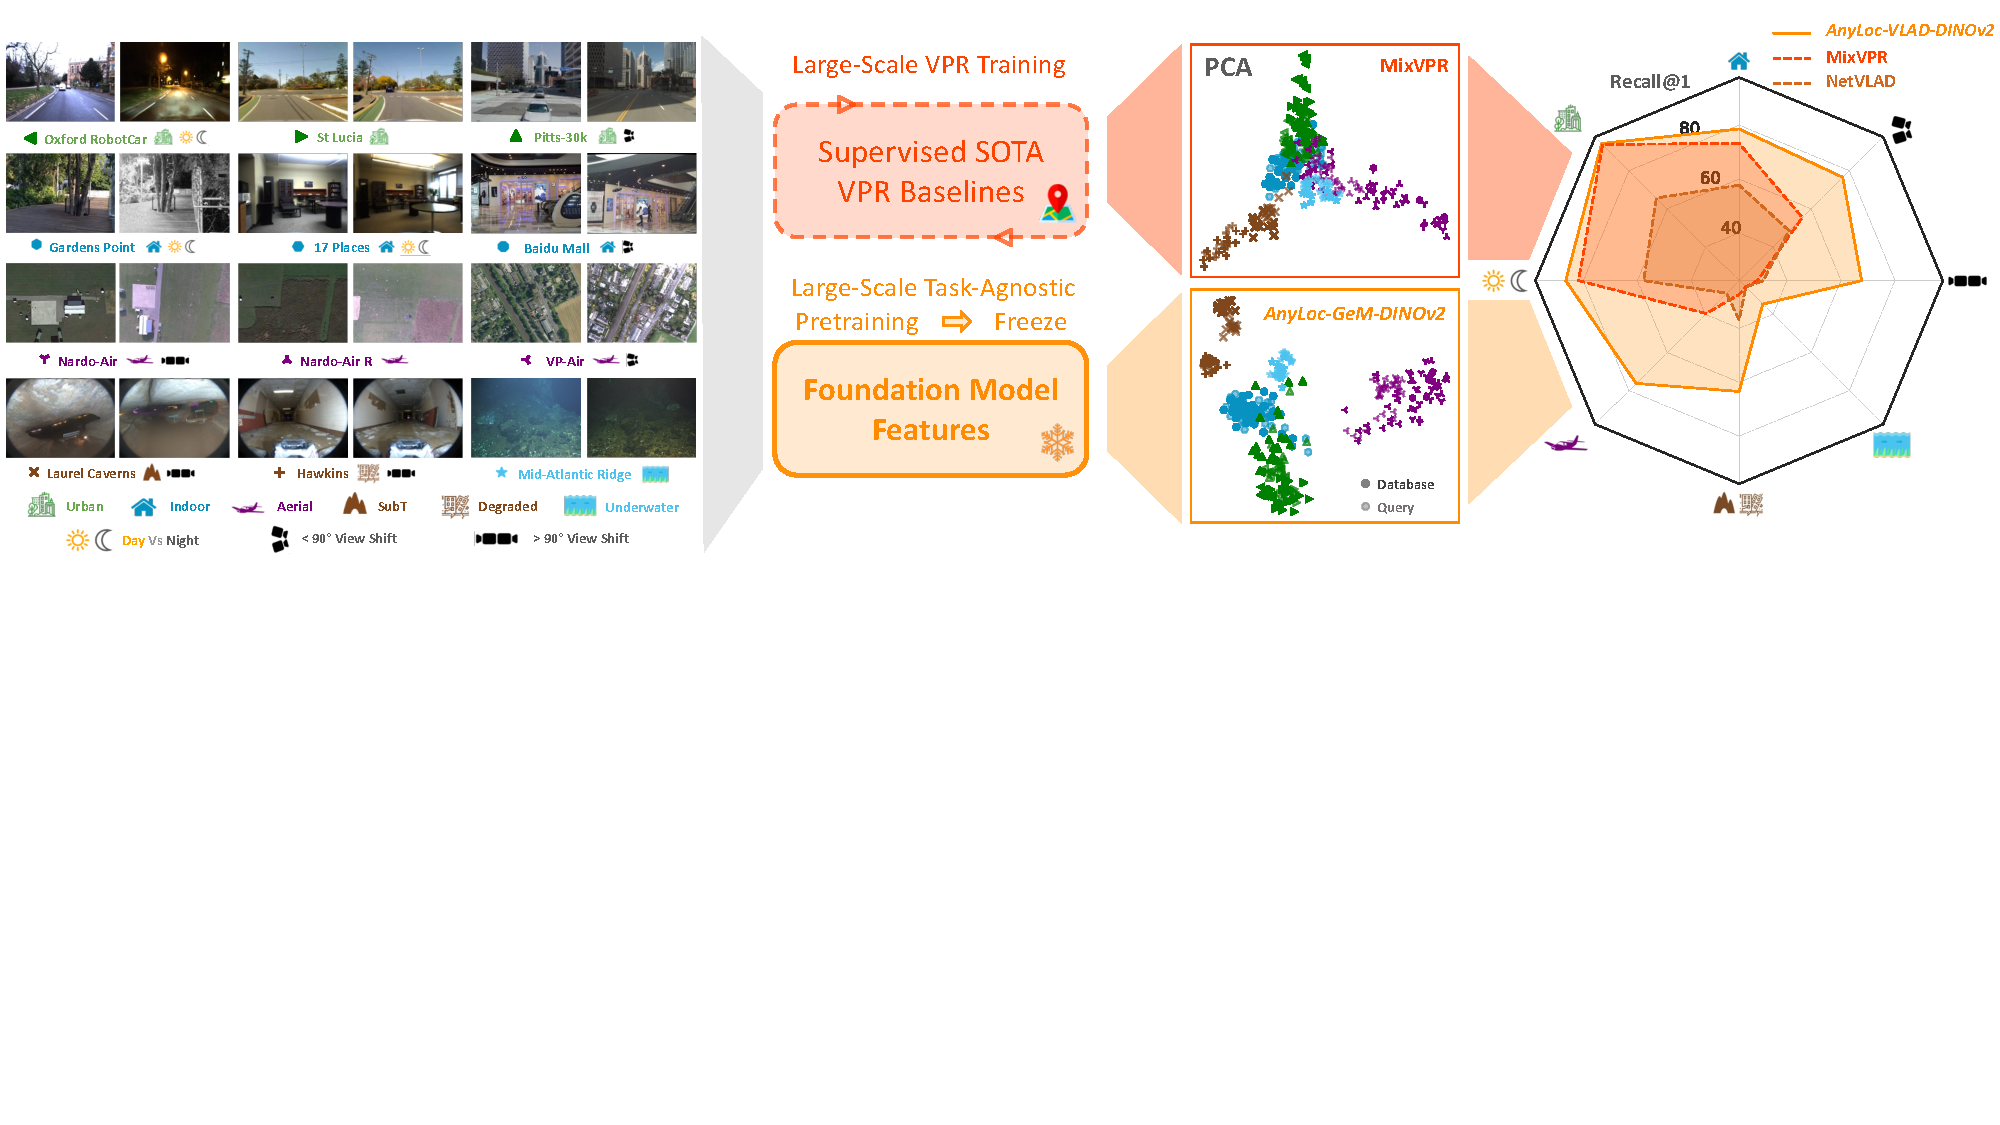
\includegraphics[trim={0cm 9.7cm 0cm 0cm},clip,
        width=0.96\linewidth]{splash.pdf}
    \caption{AnyLoc: Anywhere, Anytime, and Anyview VPR}
    \small
        \emph{Left}: Image samples from various datasets used (and the
        legend for symbols and colors). \emph{Center}: Comparing the
        PCA projections of MixVPR (a supervised baseline) and AnyLoc
        (foundation model features). \emph{Right}: VPR performance by
        the test setting. Image from \cite{Keetha2023AnyLocTU} 
        (original paper).
    \label{fig:anyloc}
\end{figure}

AnyLoc aims to perform good image retrieval (VPR) in diverse places
(anywhere), under environmental changes (anytime), and under high
viewpoint changes (anyview). For this, we extract the representations
learned by the intermediate, often penultimate, transformer layers of
DINO and DINOv2. We find that conventional feature aggregation
techniques like VLAD and GeM, described in \cref{subsec:intro-vpr},
bring significant benefit over using only the output
$\left[CLS\right]$ token of these models. Our method, when projected
to 2D, also discovers unique features that distinguish and group
datasets of similar domain, which is lacking in most recent VPR
methods (see center of \cref{fig:anyloc} for comparison with MixVPR).
The process and steps for AnyLoc are described below

\subsection{Constructing AnyLoc Pipeline}

\subsubsection{Choice of Foundation Model}

From CLIP \cite{Radford2021LearningTV}, MAE \cite{He2021MaskedAA},
DINO \cite{Caron2021EmergingPI}, and DINOv2 \cite{Oquab2023DINOv2LR},
AnyLoc employs DINO and DINOv2 ViTs for extracting features. This is
because DINO and DINOv2 are trained for representation learning
(through knowledge distillation - as described in
\cref{subsec:fm-dino} and \cref{subsec:fm-dinov2}). CLIP is trained
on alignment and is used as a benchmarking method. MAE is trained to
in-fill masked tokens (like the MIM objective in iBOT and DINOv2) and 
without any special dataset curation. We find CLIP and DINO methods
perform better than pure masked modeling of MAE.

We use \emph{DINO} and \emph{DINOv2} models for extracting
intermediate features and CLIP for benchmarking.

\subsubsection{Choosing Layer and Facet}

A vision transformer, described in \cref{subsec:vit}, patchifies an
input image and passes it through layers of transformer encoder. The
transformer encoder consists of multi-headed self-attention (MHA)
modules (alongside the normalization, residual, and FFN blocks). Each
MHA has a softmax self-attention mechanism. The input to attention
are the \texttt{query}, \texttt{key}, and \texttt{value} facets. The
output of each transformer encoder (layer) is called the 
\texttt{value} facet.

\paragraph{Description}

Let the input to the model be $\mathbf{x}^{(0)} \in \mathbb{R}^{n,
d_m}$ and the input to the $l$-th transformer encoder layer be
$\mathbf{x}^{(l-1)} \in \mathbb{R}^{n, d_m}$ (also the output of the
previous layer). This goes through a normalization layer as
\begin{math}
    \bar{\mathbf{x}}^{(l-1)} = \textup{LN}(\mathbf{x}^{(l-1)}) \in
        \mathbb{R}^{n, d_m}
\end{math}
and projected to the query, key, and value facets as follows

\begin{align}
    \mathbf{q}^l &= \bar{\mathbf{x}}^{(l-1)} \mathbf{W}_{ql} &
    \mathbf{k}^l &= \bar{\mathbf{x}}^{(l-1)} \mathbf{W}_{kl} &
    \mathbf{v}^l &= \bar{\mathbf{x}}^{(l-1)} \mathbf{W}_{vl}
\end{align}

Where $\mathbf{W}_{ql}, \mathbf{W}_{kl}, \mathbf{W}_{vl} \in
\mathbb{R}^{d_m, d_m}$ are the projection weights. These facets are
split into $h$ heads and attention is applied to each head. The output
of the attention's softmax is added with $\mathbf{x}^{(l-1)}$. This
goes through another layer normalization and FFN (in a residual) and
the final output of layer $l$ is given as $\mathbf{x}^{(l)}$.

We say $\mathbf{q}^l$ is query, $\mathbf{k}^l$ is key, $\mathbf{v}^l$
is value, and $\mathbf{x}^l$ is token facet of the $l$-th layer. Each
is of type $\mathbb{R}^{n, d_m}$ ($n$ tokens, $d_m$ dimension each)
and is a candidate for feature aggregation.

\begin{figure}
    \centering
    \begin{subfigure}[b]{0.49\textwidth}
        \centering
        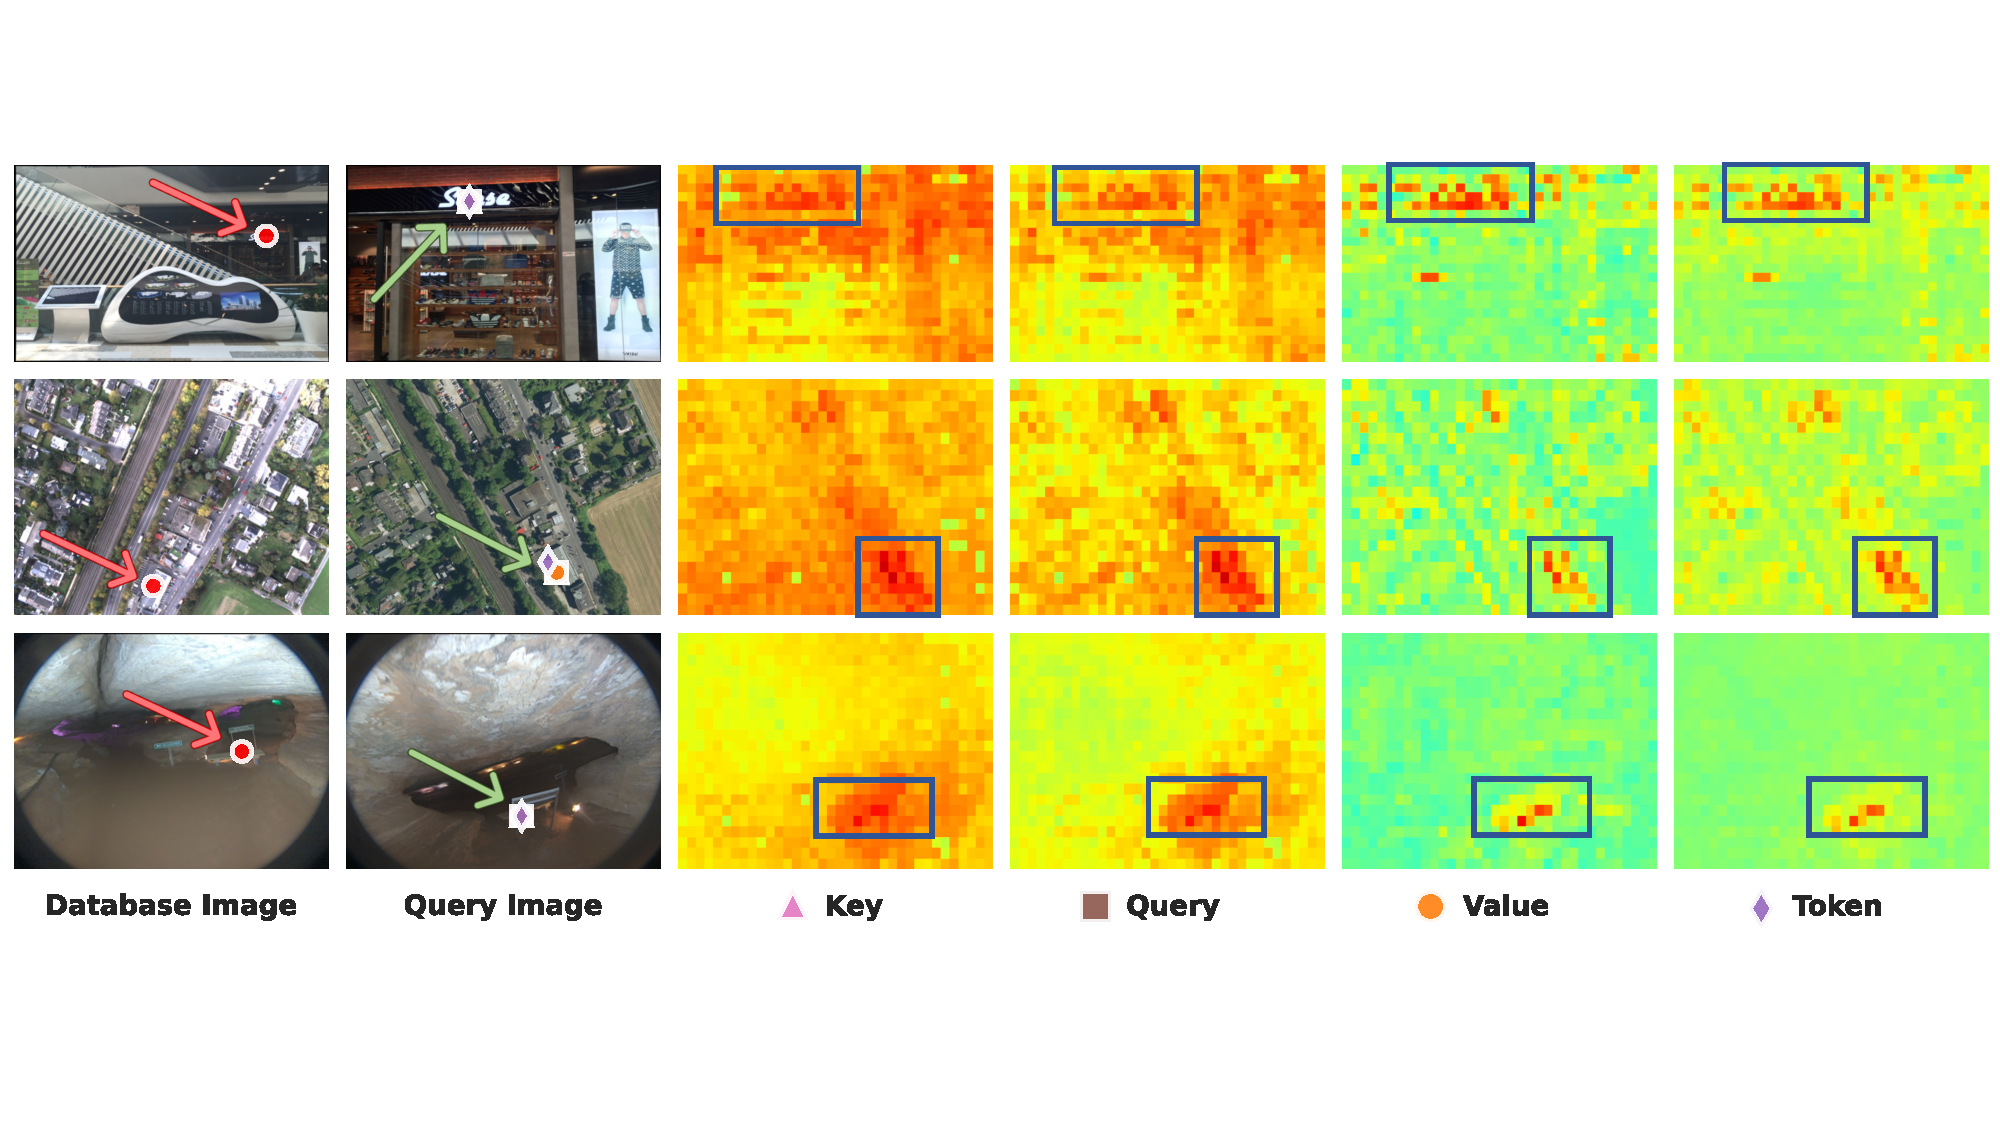
\includegraphics[trim={0cm 3.4cm 0cm 2.7cm},clip,
            width=0.95\linewidth]{facet_sim.pdf}
        \caption{Facet}
    \end{subfigure}
    \hfill
    \begin{subfigure}[b]{0.49\textwidth}
        \centering
        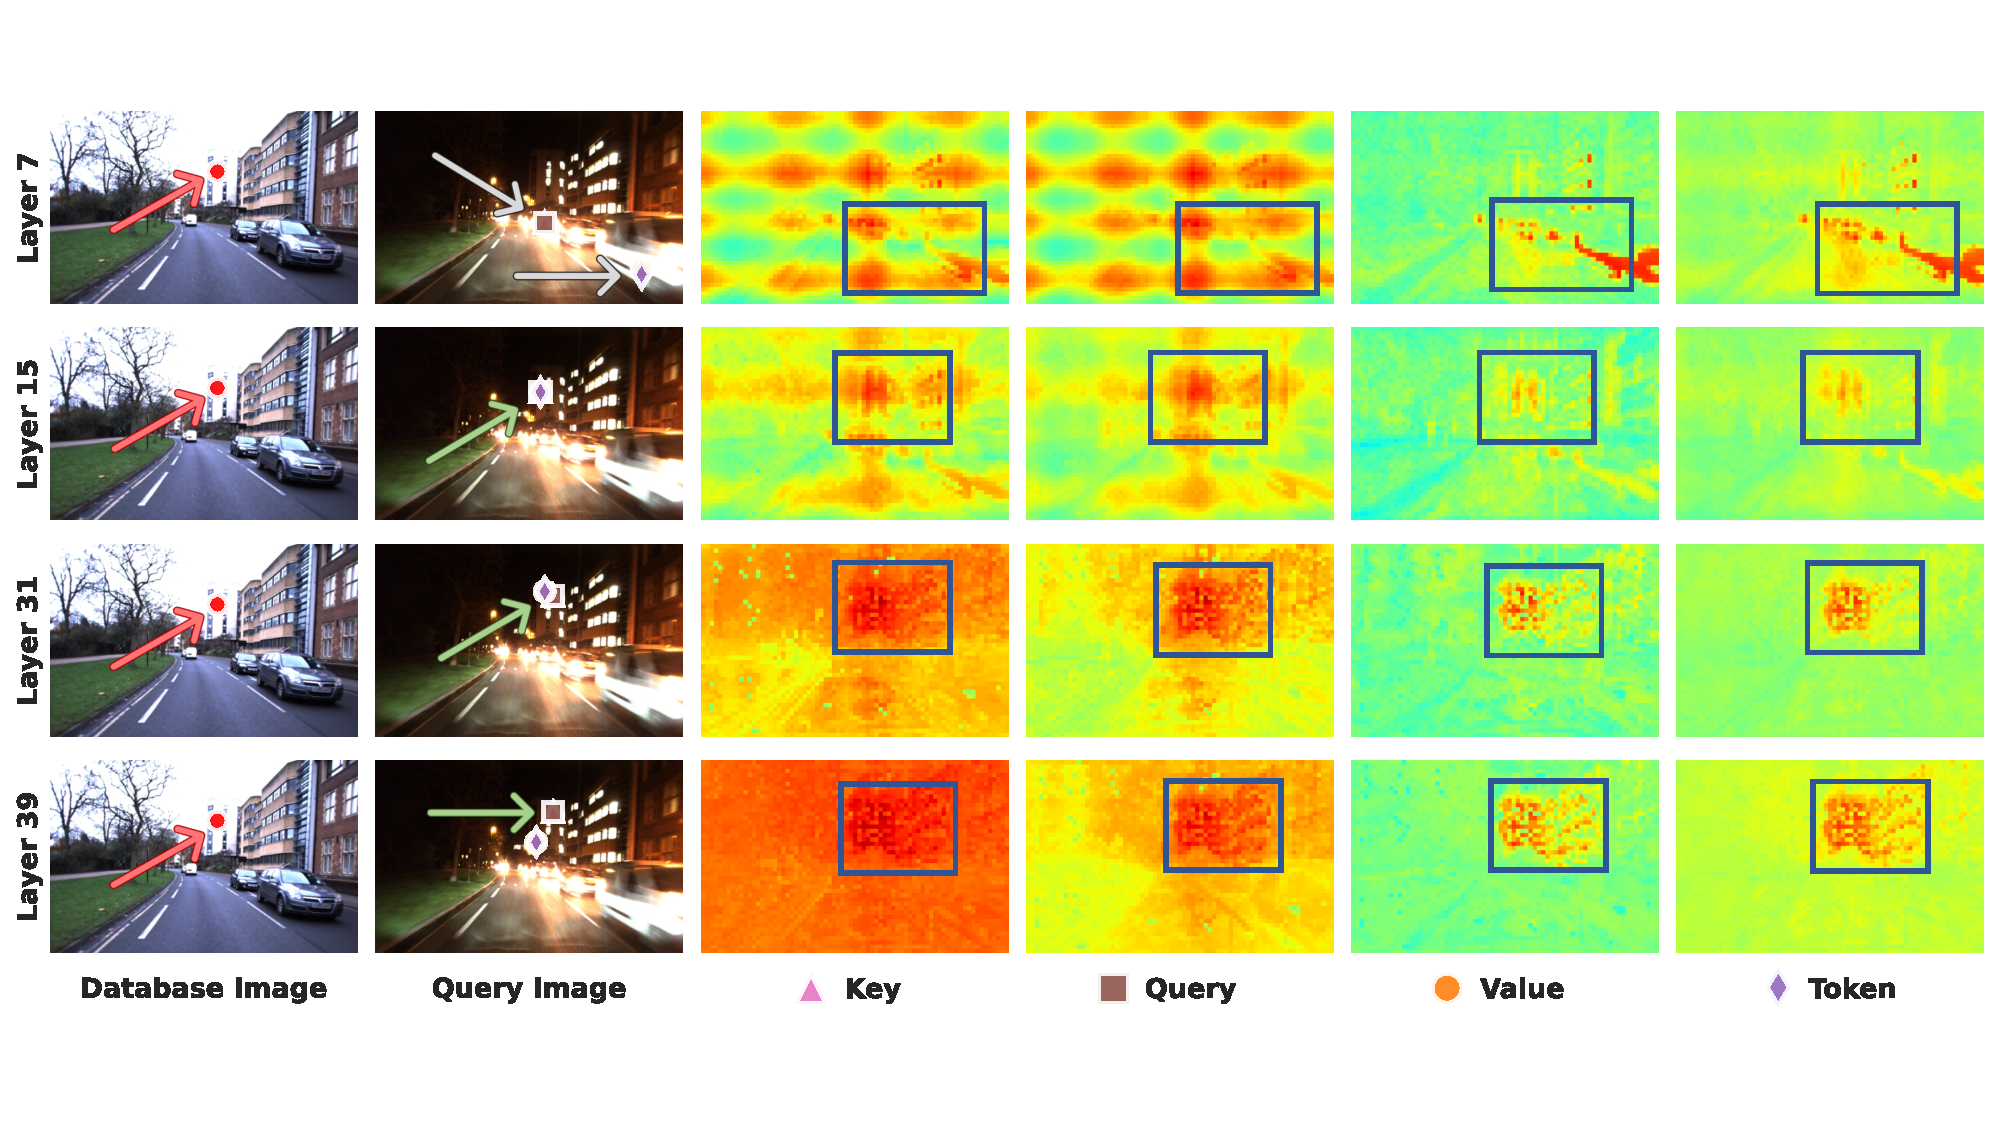
\includegraphics[trim={0cm 2.05cm 0cm 1.9cm},clip,
            width=0.95\linewidth]{facet_sim_layer_ablation.pdf}
        \caption{Layer}
    \end{subfigure}
    \caption{Facet and Layer-wise Attention Maps for DINOv2}
    \small
        \emph{Left}: Given a query point in the database image,
        various facets show different levels of contrast (with the
        most similar marker on the query image). Top has high scale
        change, middle has rotation change, and bottom has high
        perspective change. 
        \emph{Right}: A similar comparison across layers shows varying
        contrast. Notice that layer 31 shows the building (for the
        queried point in database image) with the best contrast.
    \label{fig:anyloc_facet_layer}
\end{figure}

\paragraph{Process} Given a dataset containing database and query
images, we pick a representative sample and pick a few corresponding
points. As seen in \cref{fig:anyloc_facet_layer}, a point in the left
database image is chosen and all patches (across all facets) are
extracted from the query image (on the right) and matched. A map
highlighting the similarity of each patch to the queried point is
visualized across facets and layers. The most similar patch is 
highlighted in the query image. On inspecting the similarity maps, we
can arrive at a decision on using a particular facet and layer. In the
case of \cref{fig:anyloc_facet_layer}, we choose the \texttt{value}
facet of the 31st layer (because the maps are most contrastive).


\subsubsection{Choosing Aggregation Method}

The facet features correspond to the individual patches of the image
(mostly local features with some semantic image information imbibed
due to training). These local features have to be aggregated to obtain
image-level features (also called global descriptors). These
techniques are described in \cref{subsec:intro-vpr}. We explore the 
following methods

\paragraph{VLAD} Vector of Locally Aggregated Descriptor is formed by
computing a vocabulary from a database of images, like the cluster
centers by clustering the local features. Given an image, the features
are assigned to the clusters and a residual is calculated (distance to
the cluster centers). The residuals are then aggregated for each
cluster, normalized, concatenated into one vector, and normalized
again.

Given features $\mathbf{f} \in \mathbb{R}^{n, d_m}$ (which could come 
from any facet of any layer mentioned earlier), we first get the
residual matrix $\mathbf{V} \in \mathbb{R}^{K, d_m}$

\begin{equation}
    \mathbf{V}[k, :] = \sum_{i=1}^{n} m_{i,k} (\mathbf{f}[i, :] - 
        \mathbf{c}[k, :])
\end{equation}

where $\mathbf{c} \in \mathbb{R}^{K, d_m}$ is the vocabulary of $K$
cluster centers, each $d_m$ dimensional. And $m_{i, k} = 1$ if feature
$i$ is assigned to cluster $k$ (closest to the cluster) and 0
otherwise.

\paragraph{Soft VLAD} replaces the $m_{i, k}$ with a softmax on the
distance between the feature $i$ and every cluster center $k$. This
gives distance-proportional assignment of every descriptor to every
cluster center. This is similar to the formulation of NetVLAD.

\paragraph{GeM} applies a mean pooling over the descriptors
$\mathbf{f} \in \mathbb{R}^{n, d_m}$ and gives pooled descriptor
$\mathbf{f}_G \in \mathbb{R}^{n, d_m}$ using

\begin{equation}
    \mathbf{f}_G = \left(\frac{1}{n} \sum_{i=1}^{n} \left(
            \mathbf{f}[i,:]\right)^p \right)^{\frac{1}{p}}
\end{equation}

\subsubsection{Choosing Vocabulary}

Algorithms like VLAD require a set of database images to form cluster
centers (vocabulary). We aim to characterize distinctive semantic
properties in a diverse set of environments. From \cref{fig:anyloc},
it is apparent that projecting the global descriptors of different
datasets highlights distinct domains in the latent space, allowing
us to characterize and group datasets having similar properties. 

The vocabulary is a superset (a collection of datasets) of images we
use to build database descriptors (for aggregation technique VLAD). We 
define the following types of vocabulary

\begin{itemize}
    \item \emph{Global}: Where database images from all the datasets
        are included when clustering.
    \item \emph{Structured}: Where only the database images from
        structured environments are included for clustering. These are
        outdoor and indoor datasets. These are most widely benchmarked
        in the VPR community and are from mostly human maintained
        environments.
    \item \emph{Unstructured}: Where database images from unstructured
        environments are included. These are subterranean, degraded,
        aerial, and underwater datasets. These aren't frequently
        benchmarked and remain less explored, but are important in
        scenarios like remote monitoring.
    \item \emph{Map-Specific} or dataset-specific: Where the database
        images from only the single dataset (which is being tested on)
        is used. For example, if the testing is on Oxford cars (an
        outdoor dataset), then the database images only from Oxford
        car are used to get the cluster centers for VLAD.
    \item \emph{Domain-Specific}: A domain is a collection of datasets
        with similar properties. The latent representation of AnyLoc
        descriptors allows us to discover these groups by clustering
        image descriptors from various datasets (as shown in
        \cref{fig:anyloc}). For example, for the outdoor domain, we
        use all the datasets captured in the outdoor setting.
\end{itemize}

After getting global descriptors (using aggregation techniques), we
store the descriptors from database images into a local cache and 
run similarity search for the descriptors of query images using Cosine
similarity. Note that the database cache is built offline whereas the
query's nearest neighbor lookup can be done online. 

\section{Experimental Setup}

\subsection{Datasets}

\begin{table}
    \centering
    \begin{tabular}{|ccccc||ccccc|}
        \hline
        \multicolumn{5}{|c|}{\textbf{Structured}} &
        \multicolumn{5}{|c|}{\textbf{Unstructured}} \\
        \hline
        \textbf{Dataset} & $\mathbf{N_{Db}}$ & $\mathbf{N_q}$ & 
            \textbf{Loc.} & \textbf{Type} &
        \textbf{Dataset} & $\mathbf{N_{Db}}$ & $\mathbf{N_q}$ & 
            \textbf{Loc.} & \textbf{Type} \\
        \hline
        {\color{IndoorDark} Baidu} \cite{Sun2017ADF} & 689 & 2292 & 
            10 m & \indoorChar &
        {\color{SubTDark} Hawkins} \cite{Zhao2023SubTMRSDP} & 65 & 
            101 & 8 m & \hawkinsChar \\
        {\color{IndoorDark} Gardens} \cite{Glover2021DayAN, 
            Snderhauf2015OnTP} & 200 & 200 & 5 fr & \indoorChar &
        {\color{SubTDark} Laurel} \cite{Zhao2023SubTMRSDP} & 141 & 
            112 & 8 m & \subtChar \\
        {\color{IndoorDark} 17 Places} \cite{Sahdev2016IndoorPR} & 
            406 & 406 & 5 fr & \indoorChar &
        {\color{AerialDark} Nardo-Air} \cite{He2023FoundLocVO} & 
            102 & 71 & 60 m & \aerialChar \\
        {\color{OutdoorDark} Pitts-30k} \cite{Torii2013VisualPR} & 
            10k & 6816 & 25 m & \outdoorChar &
        {\color{AerialDark} VP-Air} \cite{Schleiss2022VPAIRA} & 
            2.7k & 2.7k & 3 fr & \aerialChar \\
        {\color{OutdoorDark} St. Lucia} \cite{Warren2010UnaidedSV} & 
            1549 & 1464 & 25 m & \outdoorChar &
        {\color{UnderWaterDark} Mid-Atlantic} 
            \cite{Boittiaux2023EiffelTA} & 65 & 101 & 0.3 m & 
            \underwaterChar \\
        {\color{OutdoorDark} Oxford} \cite{Maddern20171Y1} & 191 & 
            191 & 25 m & \outdoorChar &
        &&&& \\
        \hline
    \end{tabular}
    \caption{Datasets Used for Benchmarking}
    \small
        Baidu stands for ``Baidu Mall'', Gardens stands for ``Gardens
        Point'', Laurel stands for ``Laurel Caverns'', Mid-Atlantic
        stands for ``Mid-Atlantic Ridge'' or ``Eiffel Tower''
        (underwater hydrothermal vent in the atlantic). Localization 
        radius is in meters (m) or number of frames (fm).
    \label{tab:anyloc_datasets}
\end{table}

All datasets used for benchmarking are mentioned in
\cref{tab:anyloc_datasets}, along with the type (see \cref{fig:anyloc}
for legend), number of database images $\mathbf{N_{Db}}$, number of
query images $\mathbf{N_q}$, and the localization radius used for
evaluation purposes. We choose a diverse set of structured and
unstructured datasets. Structured datasets include commonly used
indoor and outdoor datasets whereas unstructured datasets are less
commonly used, but are gaining traction in VPR because of their
challenging nature and the requirements of robotics in the near future
(subterranean and underwater datasets, for example).

To create an aerial dataset with no rotation shift between database 
and query images, we create \texttt{Nardo-Air R}, which is created by
rotating the Nardo-Air images so that they all point in the same 
direction.

\subsection{Benchmarking}

\paragraph{Baselines}

We evaluate AnyLoc against three state of the art VPR baselines:
NetVLAD \cite{Arandjelovi2015NetVLADCA}, CosPlace
\cite{Berton2022RethinkingVG}, and MixVPR \cite{Alibey2023MixVPRFM}.
To evaluate against other foundation models, we additionally propose
benchmarking CLIP \cite{Radford2021LearningTV}, DINO
\cite{Caron2021EmergingPI}, and DINOv2 \cite{Oquab2023DINOv2LR} using
their $\left[CLS\right]$ token as the global image descriptor and
performing retrieval against it. For CLIP, we use the OpenCLIP
implementation trained on the LAION-5B dataset
\cite{Ilharco2021OpenCLIP, Cherti2023ReproducibleSL,
Radford2021LearningTV, Schuhmann2022LAION5BAO}, specifically, we use
the \texttt{ViT-BigG/14} model. We use \texttt{ViT-S/8} (DeIT
implementation) for DINO and \texttt{ViT-G/14} for DINOv2.

\paragraph{Model Specifications}

For \emph{AnyLoc-VLAD-DINO}, we perform VLAD aggregation over DINO
features extracted from layer 9, \texttt{key} facet, of the
\texttt{ViT-S/8} (DeIT) model. For \emph{AnyLoc-VLAD-DINOv2}, we
perform VLAD over DINOv2 features from layer 31, \texttt{value} facet,
of the \texttt{ViT-G/14} model. For \emph{AnyLoc-GeM-DINOv2}, we
extract the same features as in the VLAD version, but perform GeM
pooling instead of VLAD aggregation.

For \emph{DINO}, the descriptor dimension for ViT-S (DeIT) is $d_m =
384$ (for each patch), and VLAD clustering is used with $K = 128$
clusters, giving a total output dimension of $384 \times 128 = 49152$.
For \emph{DINOv2}, the descriptor dimension for ViT-G/14 is $d_m =
1536$ and we use $K = 32$ clusters, giving the VLAD output dimension
$1536 \times 32 = 49152$. We additionally down-sample these global
descriptors using principal component analysis (PCA). We fit the PCA
(estimate the parameters) using only the database images, which is
done offline. The same (cached) projection parameters are used on the
query images (which are fed online). We project the dimensionality
from $49152$ to $512$ in \emph{AnyLoc-VLAD-DINO-PCA} and
\emph{AnyLoc-VLAD-DINOv2-PCA} methods.

\subsection{Evaluation}

We use the widely used \texttt{Recall@N} metric to evaluate image
retrieval (VPR) performance on each dataset. Recall@N (or
$\textup{R@N}$) is defined as the percentage of queries that have a
correct retrieval in the top-N closest retrieved database images. A
good VPR method should have high recall at low `N' value. As `N'
increases, the recall of a particular method also increases (as it is
more likely to get a correct retrieval if it's matching against more
retrieved images). We use `R@1' (top-1 retrieved) and `R@5' (top-5
retrieved) to compare all methods.

\section{Results}

\begin{table}
\centering
\begin{tabular}{|l|cc|cc|cc|cc|}
    \hline
    \multirow{3}{*}{Methods} 
    & \multicolumn{2}{|c|}{\color{IndoorDark} \textbf{Baidu Mall}} &
    \multicolumn{2}{|c|}{\color{IndoorDark} \textbf{Gardens Point}} &
    \multicolumn{2}{|c|}{\color{IndoorDark} \textbf{17 Places}} &
    \multicolumn{2}{|c|}{\textit{Average}} \\
    & \multicolumn{2}{|c|}{\indoorChar \viewpointChar} & 
    \multicolumn{2}{|c|}{\indoorChar \lightingChar} &
    \multicolumn{2}{|c|}{\indoorChar \lightingChar} & & \\
    & R@1 & R@5 & R@1 & R@5 & R@1 & R@5 & R@1 & R@5 \\
    \hline
    NetVLAD \cite{Arandjelovi2015NetVLADCA} & 53.1 & 70.5 & 58.5 & 
        85.0 & 61.6 & 77.8 & 57.73 & 77.76 \\
    CosPlace \cite{Berton2022RethinkingVG} & 41.6 & 55.0 & 74.0 & 
        94.5 & 61.1 & 76.1 & 58.9 & 75.2 \\
    MixVPR \cite{Alibey2023MixVPRFM} & 64.4 & 80.3 & 91.5 & 96.0 &
        63.8 & 78.8 & 73.23 & 85.03 \\
    \hdashline
    CLIP-\texttt{CLS} \cite{Radford2021LearningTV} & 56.0 & 71.6 & 
        42.5 & 74.5 & 59.4 & 77.6 & 52.63 & 74.56 \\
    DINO-\texttt{CLS} \cite{Caron2021EmergingPI} & 48.3 & 65.1 & 
        78.5 & 95.0 & 61.8 & 76.4 & 62.86 & 78.83 \\
    DINOv2-\texttt{CLS} \cite{Oquab2023DINOv2LR} & 49.2 & 64.6 &
        71.5 & 96.0 & 61.8 & 78.8 & 60.83 & 79.8 \\
    \hdashline
    AnyLoc-GeM-DINOv2 & 50.1 & 70.6 & 88.0 & 97.5 & 63.6 & 79.6 & 
        67.23 & 82.56 \\
    AnyLoc-VLAD-DINO & 61.2 & 78.3 & 95.0 & \underline{98.5} & 63.8 & 
        78.8 & \underline{73.33} & 85.2 \\
    AnyLoc-VLAD-DINO-PCA & 62.3 & 81.2 & 91.5 & \textbf{99.5} & 63.3 &
        78.8 & 72.36 & 86.5 \\
    \textbf{AnyLoc-VLAD-DINOv2} & \textbf{75.2} & \underline{87.6} & 
        \underline{95.5} & \textbf{99.5} & \textbf{65.0} & 
        \underline{80.5} & \textbf{78.56} & \underline{89.2} \\
    \textbf{AnyLoc-VLAD-DINOv2-PCA} & \underline{74.9} & 
        \textbf{89.4} & \textbf{96.0} & \textbf{99.5} & 
        \underline{64.8} & \textbf{81.0} & \textbf{78.56} & 
        \textbf{89.96} \\
    \hline
\end{tabular}
\caption{AnyLoc Benchmarking on Indoor Datasets}
\small
    Performance of methods on indoor datasets. \emph{Top}: Common VPR
    baselines, \emph{middle}: foundation model global descriptors
    (using CLS token), \emph{bottom}: our AnyLoc methods. The best is
    shown in \textbf{bold}, and the second best is shown in 
    \underline{underline}.
\label{tab:anyloc_bench_indoor}
\end{table}

\begin{table}
\centering
\begin{tabular}{|l|cc|cc|cc|cc|}
    \hline
    \multirow{3}{*}{Methods} 
    & \multicolumn{2}{|c|}{\color{OutdoorDark} \textbf{Pitts-30k}} &
    \multicolumn{2}{|c|}{\color{OutdoorDark} \textbf{St. Lucia}} &
    \multicolumn{2}{|c|}{\color{OutdoorDark} \textbf{Oxford}} &
    \multicolumn{2}{|c|}{\textit{Average}} \\
    & \multicolumn{2}{|c|}{\outdoorChar \viewpointChar} &
    \multicolumn{2}{|c|}{\outdoorChar} & 
    \multicolumn{2}{|c|}{\outdoorChar \lightingChar} & & \\
    & R@1 & R@5 & R@1 & R@5 & R@1 & R@5 & R@1 & R@5 \\
    \hline
    NetVLAD \cite{Arandjelovi2015NetVLADCA} & 86.1 & 92.7 & 57.9 & 
        73.0 & 57.6 & 79.1 & 67.2 & 81.6 \\
    CosPlace \cite{Berton2022RethinkingVG} & \underline{90.4} & 
        \textbf{95.7} & \underline{99.6} & \underline{99.9} & 95.3 & 
        \underline{99.5} & \textbf{95.1} & 98.36 \\
    MixVPR \cite{Alibey2023MixVPRFM} & \textbf{91.5} & 
        \underline{95.5} & \textbf{99.7} & \textbf{100} & 92.7 & 
        \underline{99.5} & \underline{94.63} & 98.33 \\
    \hdashline
    CLIP-\texttt{CLS} \cite{Radford2021LearningTV} & 55.0 & 77.2 & 
        62.7 & 80.7 & 46.6 & 60.7 & 54.76 & 72.86 \\
    DINO-\texttt{CLS} \cite{Caron2021EmergingPI} & 70.1 & 86.4 & 
        45.2 & 64.0 & 20.4 & 46.6 & 42.23 & 65.66 \\
    DINOv2-\texttt{CLS} \cite{Oquab2023DINOv2LR} & 78.3 & 91.1 & 
        78.6 & 89.7 & 47.1 & 58.1 & 68 & 79.63 \\
    \hdashline
    AnyLoc-GeM-DINOv2 & 77.0 & 87.3 & 76.9 & 89.3 & 92.2 & 97.9 & 
        82.03 & 91.5 \\
    AnyLoc-VLAD-DINO & 83.4 & 92.0 & 88.5 & 94.9 & 82.2 & 99.0 & 
        84.7 & 95.3 \\
    AnyLoc-VLAD-DINO-PCA & 82.8 & 90.8 & 87.6 & 94.3 & 82.7 & 96.3 &
        84.36 & 93.8 \\
    \textbf{AnyLoc-VLAD-DINOv2} & 87.7 & 94.7 & 96.2 & 98.8 & 
        \textbf{99.5} & \textbf{100} & 94.46 & 97.83 \\
    \textbf{AnyLoc-VLAD-DINOv2-PCA} & 86.9 & 93.8 & 96.4 & 99.5 & 
        \underline{96.9} & \textbf{100} & 93.4 & 97.76 \\
    \hline
\end{tabular}
\caption{AnyLoc Benchmarking on Outdoor Datasets}
\small
    Performance of methods on outdoor datasets. \emph{Top}: Common VPR
    baselines, \emph{middle}: foundation model global descriptors
    (using CLS token), \emph{bottom}: our AnyLoc methods. The best is
    shown in \textbf{bold}, and the second best is shown in 
    \underline{underline}.
\label{tab:anyloc_bench_outdoor}
\end{table}

\begin{table}
\centering
\begin{tabular}{|l|cc|cc|cc|cc|}
    \hline
    \multirow{3}{*}{Methods} 
    & \multicolumn{2}{|c|}{\color{AerialDark} \textbf{Nardo-Air}} &
    \multicolumn{2}{|c|}{\color{AerialDark} \textbf{Nardo-Air R}} &
    \multicolumn{2}{|c|}{\color{AerialDark} \textbf{VP-Air}} &
    \multicolumn{2}{|c|}{\textit{Average}} \\
    & \multicolumn{2}{|c|}{\aerialChar \oppositeChar} &
    \multicolumn{2}{|c|}{\aerialChar} & 
    \multicolumn{2}{|c|}{\aerialChar \viewpointChar} & & \\
    & R@1 & R@5 & R@1 & R@5 & R@1 & R@5 & R@1 & R@5 \\
    \hline
    NetVLAD \cite{Arandjelovi2015NetVLADCA} & 19.7 & 39.4 & 60.6 & 
        85.9 & 6.4 & 17.7 & 28.9 & 47.66  \\
    CosPlace \cite{Berton2022RethinkingVG} & 0 & 1.4 & 
        \underline{91.6} & \textbf{100} & 8.1 & 14.2 & 33.23 & 
        38.53 \\
    MixVPR \cite{Alibey2023MixVPRFM} & 32.4 & 42.2 & 76.1 & 
        \underline{98.6} & 10.3 & 18.3 & 39.6 & 53.03 \\
    \hdashline
    CLIP-\texttt{CLS} \cite{Radford2021LearningTV} & 42.2 & 70.4 & 
        62.0 & 97.2 & 36.6 & 52.8 & 46.93 & 73.46 \\
    DINO-\texttt{CLS} \cite{Caron2021EmergingPI} & 57.8 &
        \underline{90.1} & 84.5 & \textbf{100} & 24.0 & 38.4 & 55.43 &
        76.16 \\
    DINOv2-\texttt{CLS} \cite{Oquab2023DINOv2LR} & \underline{73.2} &
        88.7 & 71.8 & 91.6 & \underline{45.2} & \underline{59.9} &
        \underline{63.4} & \underline{80.06} \\
    \hdashline
    AnyLoc-GeM-DINOv2 & \textbf{76.1} & 83.1 & 57.8 & 97.2 & 38.3 &
        53.8 & 57.4 & 78.03 \\
    AnyLoc-VLAD-DINO & 43.7 & 54.9 & \textbf{94.4} & \textbf{100} &
        17.8 & 28.7 & 51.96 & 61.2 \\
    \textbf{AnyLoc-VLAD-DINOv2} & \textbf{76.1} & \textbf{94.4} & 
        85.9 & \textbf{100} & \textbf{66.7} & \textbf{79.2} &
        \textbf{76.23} & \textbf{91.2} \\
    \hline
\end{tabular}
\caption{AnyLoc Benchmarking on Aerial Datasets}
\small
    Performance of methods on aerial datasets. \emph{Top}: Common VPR
    baselines, \emph{middle}: foundation model global descriptors
    (using CLS token), \emph{bottom}: our AnyLoc methods. The best is
    shown in \textbf{bold}, and the second best is shown in 
    \underline{underline}. Note that aerial datasets are also included
    in our classification of unstructured datasets. However, they also
    form a domain of their own, hence these results are in a separate
    table.
\label{tab:anyloc_bench_aerial}
\end{table}

\begin{table}
\centering
\begin{tabular}{|l|cc|cc|cc|}
    \hline
    \multirow{3}{*}{Methods} 
    & \multicolumn{2}{|c|}{\color{SubTDark} \textbf{Hawkins}} &
    \multicolumn{2}{|c|}{\color{SubTDark} \textbf{Laurel Caverns}} &
    \multicolumn{2}{|c|}{\color{UnderWaterDark} 
        \textbf{Mid-Atlantic Ridge}} \\
    & \multicolumn{2}{|c|}{\hawkinsChar \oppositeChar} &
    \multicolumn{2}{|c|}{\subtChar \oppositeChar} & 
    \multicolumn{2}{|c|}{\underwaterChar} \\
    & R@1 & R@5 & R@1 & R@5 & R@1 & R@5 \\
    \hline
    NetVLAD \cite{Arandjelovi2015NetVLADCA} & 34.8 & 71.2 & 39.3 & 
        71.4 & 25.7 & 53.5 \\
    CosPlace \cite{Berton2022RethinkingVG} & 31.4 & 59.3 & 24.1 & 
        47.3 & 20.8 & 40.6 \\
    MixVPR \cite{Alibey2023MixVPRFM} & 25.4 & 60.2 & 29.5 & 67.0 & 
        25.7 & 60.4 \\
    \hdashline
    CLIP-\texttt{CLS} \cite{Radford2021LearningTV} & 33.0 & 67.0 & 
        36.6 & 66.1 & 25.7 & 51.5 \\
    DINO-\texttt{CLS} \cite{Caron2021EmergingPI} & 46.6 & \underline{84.8} & 
        41.1 & 57.1 & 27.7 & 49.5 \\
    DINOv2-\texttt{CLS} \cite{Oquab2023DINOv2LR} & 28.0 & 62.7 & 
        40.2 & 65.2 & 24.8 & 48.5 \\
    \hdashline
    AnyLoc-GeM-DINOv2 & \underline{53.4} & 83.9 & 58.9 & 
        \underline{86.6} & 14.8 & 49.5 \\
    AnyLoc-VLAD-DINO & 48.3 & \underline{84.8} & \underline{57.1} & 
        79.5 & \textbf{41.6} & \textbf{66.3} \\
    \textbf{AnyLoc-VLAD-DINOv2} & \textbf{65.2} & \textbf{94.1} & 
        \textbf{61.6} & \underline{90.2} & \underline{34.6} & 
        \underline{61.4} \\
    \hline
\end{tabular}
\caption{AnyLoc Benchmarking on Unstructured Datasets}
\small
    Performance of methods on unstructured datasets (outside aerial
    domain). \emph{Top}: Common VPR baselines, \emph{middle}:
    foundation model global descriptors (using CLS token),
    \emph{bottom}: our AnyLoc methods. The best is shown in
    \textbf{bold}, and the second best is shown in
    \underline{underline}.
\label{tab:anyloc_bench_unstruct}
\end{table}

\subsection{Overall}

The results for indoor, outdoor, aerial, and remaining unstructured
datasets are presented in \cref{tab:anyloc_bench_indoor},
\cref{tab:anyloc_bench_outdoor}, \cref{tab:anyloc_bench_aerial}, and
\cref{tab:anyloc_bench_unstruct} respectively. 

It is interesting to note that even with a $96\times$ reduction
descriptor dimension through PCA, AnyLoc methods hardly loose any
performance. This robustness to dimensionality reduction could be
attributed to regularization techniques during training these
foundation models, promoting the learning of efficient representations
across channels. This robustness could also be a reason why AnyLoc can
easily separate and group datasets of different domains in the 2D PCA 
projection in \cref{fig:anyloc} whereas MixVPR struggles to separate
the data in such a low dimension.

AnyLoc methods perform much better than the benchmark for the indoor
domain. Interestingly, the \texttt{CLS} baselines of foundation models
are competitive with conventional VPR baselines out-of-the-box. Simple
aggregation techniques over DINO and DINOv2 give a new
state-of-the-art model in this category.

Most \texttt{CLS} baselines fail in outdoor settings, due to not being
explicitly trained on outdoor data; only DINOv2 has Google Landmarks
so it performs relatively better than DINO and CLIP. However, adding
conventional aggregation techniques to foundation model baselines 
bring them at-par with the VPR baselines that are explicitly trained
for outdoor VPR. AnyLoc DINOv2 methods, perform better than VPR 
baselines in the presence of day-vs-night change (Oxford).

Traditional VPR methods, though being trained on ourdoor data, perform
poorly on aerial data. This could be because they fail to generalize
on top-view images. Upon visual inspection of retrievals, we find
that CosPlace retrieves a particular fixed set of reference images
for almost all query images (giving poor results on Nardo-Air).

Foundation models and AnyLoc methods are significantly better than VPR
baselines on aerial datasets. They set a new state-of-the-art, with
the worst performer (CLIP-\texttt{CLS}) beating the best traditional
VPR method (MixVPR) by more than $7\%$. AnyLoc-VLAD methods,
especially with DINOv2, yield robust results that are unseen on
previous benchmarks.

The performance of AnyLoc-VLAD-DINOv2 on Laurel Caverns and
Mid-Atlantic Ridge is significantly better than VPR baselines (and
even foundation models), showcasing the utility of the methods even 
under conditions where distinct keypoints are few and when there is a 
high viewpoint change involved.

\subsection{Vocabulary Domain Ablation}

\begin{table}
    \centering
    \begin{tabular}{|l|ccc|}
        \hline
        \multirow{2}{*}{\textbf{Vocabulary Type}} & 
            {\color{IndoorDark}\textbf{Indoor}} &
            {\color{OutdoorDark}\textbf{Outdoor}} &
            {\color{AerialDark}\textbf{Aerial}} \\
        & \indoorChar & \outdoorChar & \aerialChar \\
        \hline
        Global & 77.0 & 93.9 & 57.1 \\
        Structured & 77.0 & 93.3 & 56.4 \\
        Unstructured & 74.8 & 89.0 & 75.8 \\
        Map-Specific & 78.0 & 92.3 & 62.9 \\
        Domain-Specific & \textbf{78.6} & \textbf{94.4} & 
            \textbf{76.2} \\
        \hline
    \end{tabular}
    \caption{Vocabulary Analysis using AnyLoc-VLAD-DINOv2}
    \small
        Different vocabularies (first column) are tried against
        different dataset domains (heading of next three columns).
        The `R@1' is calculated and averaged across the domains. The
        best results are in \textbf{bold}
    \label{tab:anyloc_vocab}
\end{table}

We study the effect of using different vocabularies (collection of
datasets) for different deployment scenarios. The overall results are
shown in \cref{tab:anyloc_vocab}. It is evident that using the
domain-specific vocabulary for each domain gives the best result; that
is, using database images across various indoor datasets is the best
option to test on an indoor dataset (even better than using database
images only from the single dataset being tested). This shows good
knowledge transfer abilities of AnyLoc. Interestingly, using
unstructured vocabulary for structured domains (indoor and outdoor)
degrades performance by only $4\%$, but gives significant boost to
evaluations on unstructured datasets (aerial).

\subsubsection{Vocabulary Transfer Behavior}

\begin{table}
    \centering
    \begin{tabular}{|llcc|}
        \hline
        \textbf{Vocabulary Dataset} & \textbf{Evaluation Dataset} & 
            \textbf{Map-Specific R@1} & \textbf{Vocab-Specific R@1} \\
        \hline
        \multirow{2}{*}{\color{IndoorDark} Baidu Mall (0.7k)} &
            {\color{IndoorDark} 17 Places (0.4k)} & \textbf{64.5} & 
            63.8 \\
        & {\color{IndoorDark} Gardens Point (0.2k)} & \textbf{98.0} &
            94.5 \\
        \hdashline
        \multirow{2}{*}{\color{AerialDark} VP-Air (2.7k)} &
            {\color{AerialDark} Nardo-Air (0.1k)} & 57.8 & 
            \textbf{64.8} \\
        & {\color{AerialDark} Nardo-Air R (0.1k)} & 70.4 & 
            \textbf{88.7} \\
        \hdashline
        \multirow{1}{*}{\color{OutdoorDark} Pitts-30k (10k)} &
            {\color{OutdoorDark} Oxford (0.2k)} & 94.8 & 
            \textbf{99.0} \\
        \hline
    \end{tabular}
    \caption{Vocabulary Transfer for AnyLoc-VLAD-DINOv2}
    \small
        Using a large vocabulary dataset, we test how well the cluster
        centers trained on the testing dataset (map-specific) perform
        w.r.t. those transferred form the given dataset
        (vocab-specific). The first column is the large dataset (for
        vocab testing), second column is the dataset for evaluation,
        third column is results using the evaluation dataset alone (no
        transfer), fourth column is results using transfer of vocab.
        Top row is for indoor domain, middle is for aerial, and bottom
        is for outdoor.
    \label{tab:anyloc_vocab_transfer}
\end{table}

We additionally diagnose the vocabulary transfer abilities of our 
model by using one large dataset for building vocabulary, and testing 
on other datasets of the same domain. The results for this are shown 
in \cref{tab:anyloc_vocab_transfer}. It is clear that, in case of
using vocabulary transfer from another dataset, the vocabulary dataset
should be large. Using cluster centers obtained from Pitts-30k to
evaluate Oxford gives a significant boost of more than $4\%$ (over 
using cluster centers from only Oxford).

This shows that we can save the vocabulary (cluster centers) in
long-term storage and use them based on the deployment environment.
One way to estimate the deployment environment could be to project
sample images on a template projection map containing images from
different domains, like the PCA projections by AnyLoc-GeM-DINOv2 in
\cref{fig:anyloc}.

\subsubsection{Visual Analysis of Vocabulary}

\begin{figure}
    \centering
    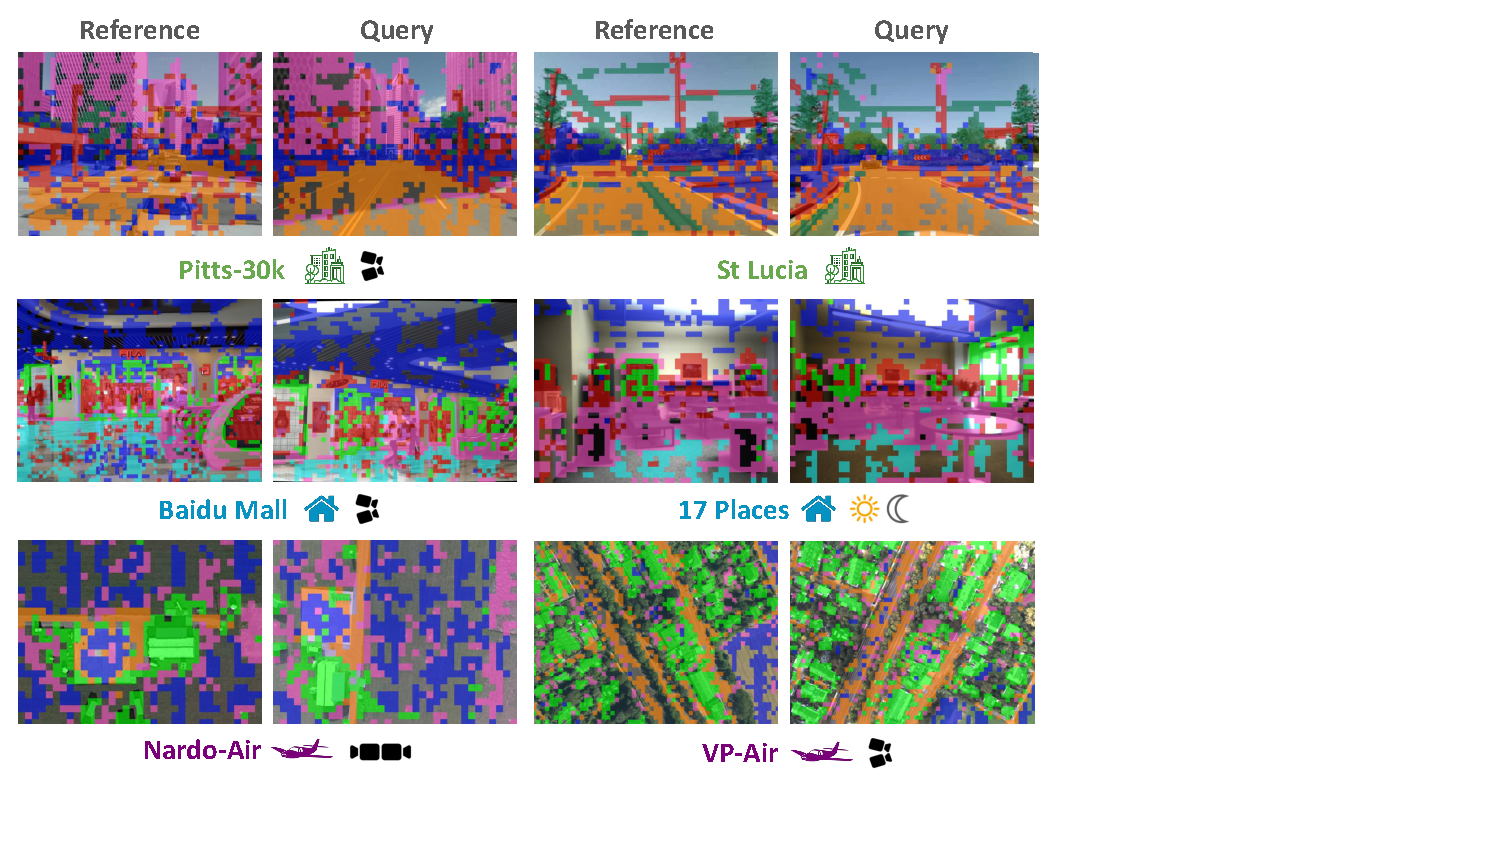
\includegraphics[trim={0cm 1.2cm 7.5cm 0cm}, clip,
        width=0.75\linewidth]{cluster_viz_domain.pdf}
    \caption{VLAD Cluster Visualizations}
    \small
        Visualizing the clusters different patches of the image belong
        to. We use domain vocabulary (clusters) for this purpose. In 
        each row, patches belonging to the same cluster have the same 
        color. Noisy clusters are not visualized for clarity.
    \label{fig:anyloc_cluster_viz}
\end{figure}

We visualize the cluster assignments in \cref{fig:anyloc_cluster_viz}.
This is done by color coding the cluster numbers and projecting the
assigned numbers (closest cluster center) to each patch (since
descriptors are patch-wise). We notice that most clusters learn (latch
onto) semantically meaningful information needed for good VPR. For
example, the buildings in aerial images (green), furniture in indoor
images (purple), and road, buildings, and horizon in outdoor images
(orange, pink, and blue respectively). For the purpose of this
experiment, we use $K = 8$ clusters.

\subsection{Design Ablation}

\begin{figure}
    \centering
    \begin{tabular}{ccc}
        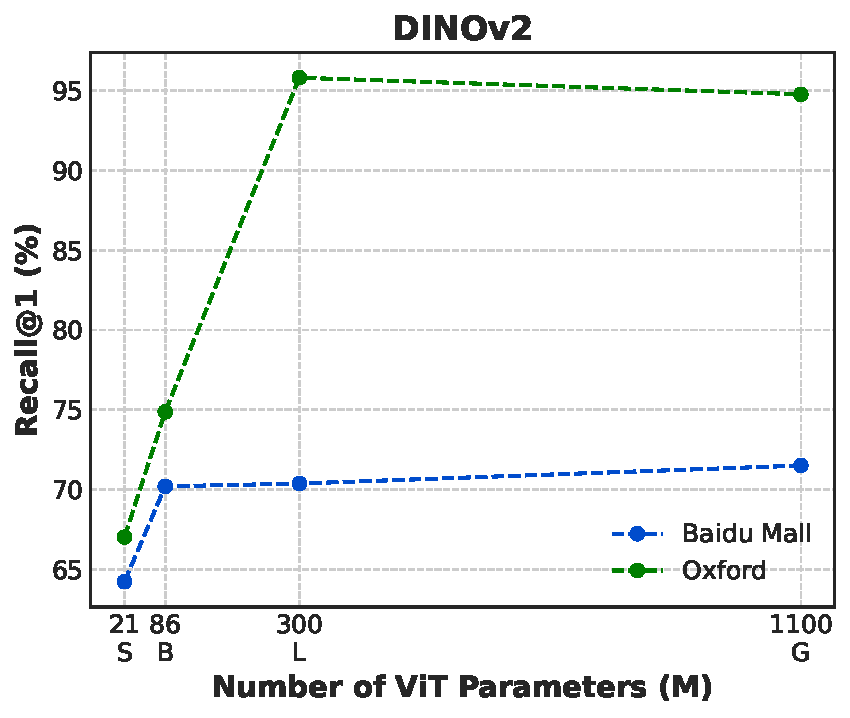
\includegraphics[trim={0.2cm 0cm 0.2cm 0cm}, clip, 
            width=0.3\linewidth]{ablations/vit_models.pdf} &
        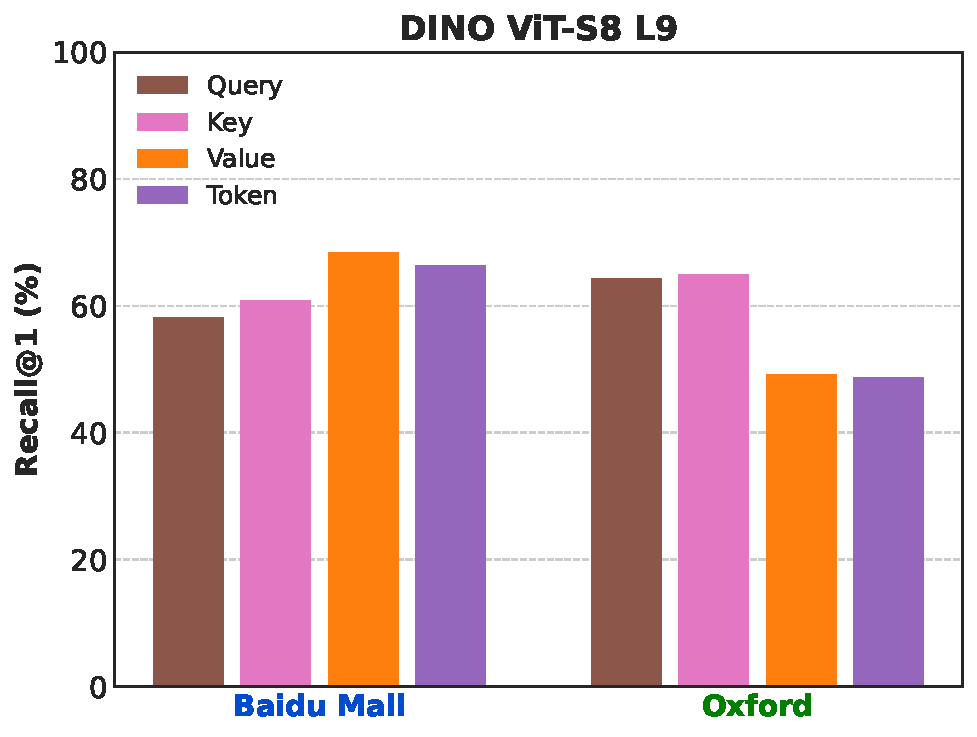
\includegraphics[trim={1cm -0.2cm 0 0}, 
            width=0.3\linewidth]{ablations/Facet_DINO_ViT_S8_L9.pdf} &
        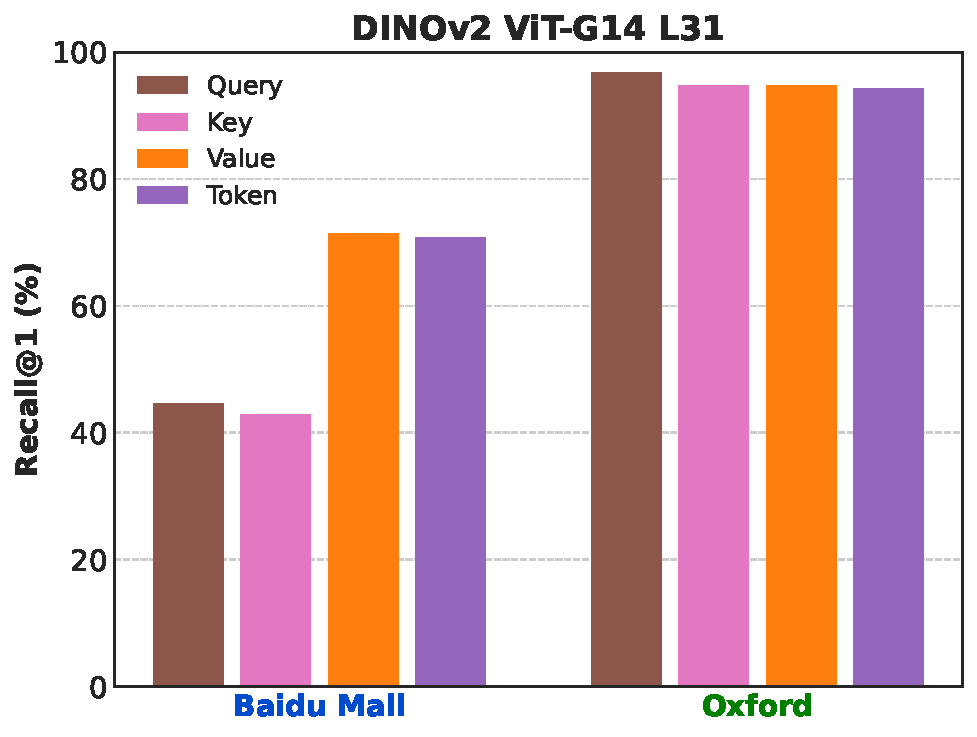
\includegraphics[trim={1cm -0.2cm 0 0}, 
            width=0.3\linewidth]{ablations/Facet_DINOv2_ViT_G14.pdf}
            \\
        (a) Model & \multicolumn{2}{c}{(b) Facet} \\
    \end{tabular}
    \begin{tabular}{cc}
        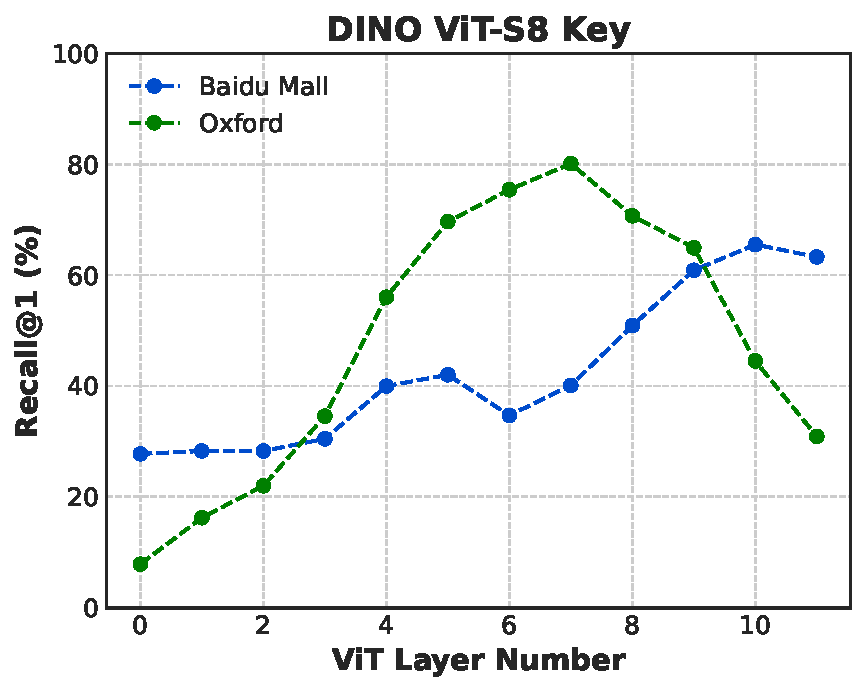
\includegraphics[trim={0.2cm 0cm 0.2cm 0cm}, clip, 
            width=0.35\linewidth]{ablations/Layer_DINO_ViT_S8_Key.pdf}
            &
        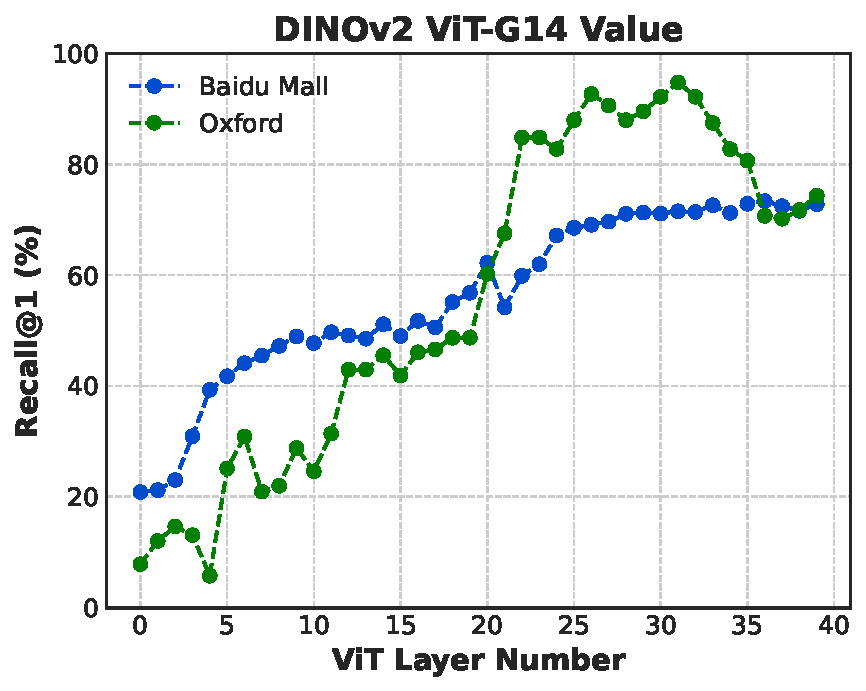
\includegraphics[trim={0.2cm 0cm 0.2cm 0cm}, clip, 
            width=0.35\linewidth]{ablations/Layer_DINOv2_ViT_G14.pdf} 
            \\
        \multicolumn{2}{c}{(c) Layer}
    \end{tabular}
    \caption{AnyLoc Design Ablations}
    \small
        (a) Performance varying by model size. (b) On average,
        \texttt{key} and \texttt{value} perform best for DINO and
        DINOv2 respectively. (c) Performance peaks at penultimate
        layers of DINO and DINOv2.
    \label{fig:anyloc_design_ablations}
\end{figure}

To better justify our choice of model parameters like layer, facet,
and pooling techniques, we run thorough ablations in
\cref{fig:anyloc_design_ablations} (tested on Baidu Mall and Oxford
datasets).

We see that using ViT-G (with 1.1B parameters) gives the best results
on the test datasets. ViT-L (with 300M parameters) gives the closest
best result, followed by ViT-B (with 86M parameters) and ViT-S (with
21M parameters). The low change when downgrading from ViT-G to ViT-L
shows that DINOv2 retains performance even after a large reduction in
parameters. This could be a result of the distillation strategy of
DINOv2 (smaller models are distilled from larger models) discussed in
\cref{subsec:fm-dinov2}.

On average, using the \texttt{key} facet for DINO and \texttt{value}
facet for DINOv2 gives the best results across dataset domains. The
layer ablations show that performance is low at the initial layers, 
peaks at the penultimate layers, and then gradually stagnates or goes
down. We believe this is because of unique representations learned
per layer. It is possible that later layers learn more meaningful
global representations at the cost of local information. As a good
middle ground, we choose \texttt{layer 9} for \texttt{DINO ViT-S/8}
and \texttt{layer 31} for \texttt{DINOv2 ViTT-G/14}.


\subsubsection{Architecture}

\begin{table}
    \centering
    \begin{tabular}{|l|ccccc|}
        \hline
        \multirow{2}{*}{\textbf{Method}} & 
            {\color{IndoorDark} Indoor} & 
            {\color{OutdoorDark} Urban} & 
            {\color{AerialDark} Aerial} & 
            {\color{SubTDark} SubT \& D} &
            {\color{UnderWaterDark} Underwater} \\
        & \indoorChar & \outdoorChar & \aerialChar & \subtChar 
            \hawkinsChar & \underwaterChar \\
        \hline
        ViT-B CosPlace & 62.9 & 80.7 & 26.3 & 26.5 & 18.8 \\
        ViT-B CosPlace VLAD & 68.5 & 82.9 & 38.4 & 37.5 & 23.8 \\
        \hdashline
        ViT-S AnyLoc-VLAD-DINO & 72.9 & 79.6 & 47.8 & 52.7 & 
            \textbf{41.6} \\
        ViT-B AnyLoc-VLAD-DINOv2 & 77.0 & 82.6 & 53.6 & 60.2 & 35.6 \\
        ViT-G AnyLoc-VLAD-DINOv2 & \textbf{78.0} & \textbf{92.3} & 
            \textbf{62.9} & \textbf{63.4} & 34.6 \\
        \hline
    \end{tabular}
    \caption{VPR Trained ViTs Vs. Self Supervised ViTs}
    \small
        Analysis of ViTs trained for VPR (top rows) versus
        self-supervised ViTs (bottom rows). Best results are in 
        \textbf{bold}. All numbers are Recall@1 percentages.
    \label{fig:anyloc_cosplace_vit}
\end{table}

We additionally investigate the affect of the architecture on recalls
in \cref{fig:anyloc_cosplace_vit}. We use the author's implementation
of GeM pooling on ViT-B's output \cite{Berton2022RethinkingVG}. We
also test this against VLAD aggregation ($K = 128$ clusters) over the
6th layer's values for CosPlace ViT-B (we found this performs best).

We find that AnyLoc gives better results than CosPlace ViT, despite 
using a smaller ViT (ViT-S). On the urban setting, since CosPlace is 
trained on it, it performs slightly better. However, we achieve the 
best performance using ViT-G AnyLoc-VLAD-DINOv2.

\subsubsection{Pooling Methods}

\begin{table}
    \centering
    \begin{tabular}{|l|ccc|ccc|}
        \hline
        \multirow{2}{*}{\textbf{Aggregation Methods}} & 
            \multicolumn{3}{c|}{DINO} & \multicolumn{3}{c|}{DINOv2} \\
        & {\color{IndoorDark} Baidu $\uparrow$} & 
        {\color{OutdoorDark} Oxford $\uparrow$} & Dim $\downarrow$ & 
            {\color{IndoorDark} Baidu $\uparrow$} & 
        {\color{OutdoorDark} Oxford $\uparrow$} & Dim $\downarrow$ \\
        \hline
        Global Average Pooling (GAP) & 29.6 & 28.8 & \textbf{384} & 
            41.6 & 78.5 & \textbf{1536} \\
        Global Max Pooling (GMP) & 34.9 & 38.2 & \textbf{384} & 64.4 &
            74.9 & \textbf{1536} \\
        Generalized Mean Pooling (GeM) & 34.7 & 47.6 & \textbf{384} &
            50.1 & 92.2 & \textbf{1536} \\
        Soft Assignment VLAD & 33.8 & 28.3 & 49152 & 40.3 & 82.2 &
            49152 \\
        Hard Assignment VLAD & \textbf{60.9} & \textbf{64.9} & 49152 &
            \textbf{71.5} & \textbf{94.8} & 49152 \\
        \hline
    \end{tabular}
    \caption{AnyLoc Aggregation Methods}
    \small
        Testing various feature aggregation methods for AnyLoc using
        DINO and DINOv2 features (same facet and layer as AnyLoc).
        Note that for DINOv2, through VLAD has high dimension, the PCA
        projected version has only 512 dimension. It is not included
        here for fairness. The numbers in \texttt{Dim} column are
        integers (lower is better) and the numbers in other columns
        are Recall@1 percentages (higher is better).
    \label{tab:anyloc_agg_ablation}
\end{table}

We try different pooling methods in \cref{tab:anyloc_agg_ablation}. We
find that VLAD pooling with hard cluster assignments gives the best
results, followed by GeM pooling. Surprisingly, these methods do not
perform well when using soft cluster assignments in VLAD (like in
NetVLAD). This could be because these models aren't trained for VLAD.

\section{Conclusion}

This work introduces AnyLoc, a novel general-purpose visual place
recognition (image retrieval) system achieving state-of-the-art
performance across diverse domains (indoor, aerial, unstructured)
under varying conditions (day/night, viewpoints). By leveraging
features from foundation models and unsupervised aggregation
techniques, AnyLoc outperforms existing VPR systems by up to 5\%, 35\%,
and 30\% in these domains, respectively. Notably, it demonstrates
competitive results even on outdoor environments without specific
supervision or training data, highlighting its generalizability.
Developments like AnyLoc are crucial for enabling robust robot
navigation and perception in real-world scenarios with limited or
unavailable domain-specific data.
